% !TEX root = UAV_Landing_Pad.tex
\chapter{User Stories, Backlog and Requirements}
\section{Overview}


%The overview should take the form of an executive summary.  Give the reader a feel 
%for the purpose of the document, what is contained in the document, and an idea 
%of the purpose for the system or product. 
%
% The userstories 
%are provided by the stakeholders.  You will create he backlogs and the requirements, and document here.  
%This chapter should contain 
%details about each of the requirements and how the requirements are or will be 
%satisfied in the design and implementation of the system.
%
%Below:   list, describe, and define the requirements in this chapter.  
%There could be any number of sub-sections to help provide the necessary level of 
%detail. 



The following chapter is the overview of the Landing Pad Senior Design project. The intention is to give a generalized top-level report of the project without delving too deeply into any of the technical components. The project's overall goal, stakeholder information, development requirements, and development timeline will all be covered in the following sections. Please refer to Chapter~\ref{chapterDesignAndImplementation} for a more detailed look at the project's design and implementation.





\subsection{Scope}


%What scope does this document cover?  This document would contain stakeholder information, 
%initial user stories, requirements, proof of concept results, and various research 
%task results. 

This section covers project user stories, stakeholder information, and general project requirements.


\subsection{Purpose of the System}
%What is the purpose of the system or product? 

The purpose of this project is to design a system where an Unmanned Ground Vehicle transports an Unmanned Aerial Vehicle to designated flight locations. The UAV will initiate flight off of a landing pad situated on the ground vehicle, which it will autonomously return to after flight is completed.

An Unmanned Aerial Vehicle is capable of collecting sensor data from above a target site and communicate that data back to a home location. The battery life on a standard quad copter does not support extended flight times, so having a UAV fly over a vast expanse of an area is not feasible. The intended purpose of the ground vehicle is to transport the UAV to different flight locations while charging the air vehicle during transportation.

\section{ Stakeholder Information}

The following section details the stakeholders in this project, including the Product Owner, the Scrum Master, potential Investors, and the various roles of the developers involved with the project.
%This section would provide the basic description of all of the stakeholders for 
%the project.  Who has an interest in the successful and/or unsuccessful completion 
%of this project? 


\subsection{Customer or End User (Product Owner)}
%Who?  What role will they play in the project?  Will this person or group manage 
%and prioritize the product backlog?  Who will they interact with on the team to 
%drive product backlog priorities if not done directly? 

The product owner of this project is Dr. Jeff McGough. Our team has a weekly meetings with Dr. McGough every Tuesday at 8AM during the first semester of Senior Design and every Thursday at 10AM during the second semester of Senior Design. All project features and product backlog prioritization is conducted by Dr. McGough during these meetings.


\subsection{Management or Instructor (Scrum Master)}
%Who?  What role will they play in the project?  Will the Scrum Master drive the 
%Sprint Meetings? 

The Scrum Master for the Landing Pad project is Julian Anthony Brackins. The tasks laid out for Julian besides being a standard developer on the team is to facilitate and drive Sprint Meetings, and coordinate meeting times for the team to collaborate and work on the project outside of class. Julian is also in charge of coordinating the design document for senior design, as well as the sprint recap presentations and poster for the Senior Design Fair.


\subsection{Investors}
%Are there any?  Who?  What role will they play? 
As of right now, there currently are no outside investors. The intended goal of this project is to find investors in the search and rescue field that would be interested in using our integrated UAV and UGV system to assist with finding missing persons in situations deemed unsafe for human involvement, including forest fires and other natural disasters.

\subsection{Developers}
%Who?  Is there a defined project manager, developer, tester, designer, architect, 
%etc.? 
With the size of our project, each of our team members has a specified role or multiple roles in the project:
\begin{itemize}
	\item[] Colter Assman
		\begin{itemize}
			\item \textbf{UAV Specialist}. In charge of designing software routine for manual override on the UAV, facilitating fully autonomous flight. Also tasked with general software and hardware component integration on the UAV.
		\end{itemize}
	\item[] Julian Brackins
		\begin{itemize}
			\item \textbf{Scrum Master}. Coordinates team meetings and code reviews, lead author for design document, presentations, and poster.
			\item \textbf{Craft Orientation Specialist}. Using OpenCV to design an object tracking system for the UAV to recognize and navigate towards the landing pad.
		\end{itemize}
	\item[] Samuel Carroll
		\begin{itemize}
			\item \textbf{Navigation Specialist}. Designing an obstacle avoidance routine for the ground vehicle using point cloud data.
			\item \textbf{UGV Specialist}. Assisting with the construction of the new unmanned ground vehicle.
		\end{itemize}
	\item[] Hafiza Farzami
		\begin{itemize}
			\item \textbf{Control Panel Specialist}. Designer for a front-end display panel used to handle manual ground vehicle control and view incoming sensor data from the ground vehicle and aerial vehicle.
			\item  \textbf{Craft Orientation Specialist}. Using ROS to design an AR tag tracking routine to determine UAV pose, distance, and orientation in relation to the landing pad.
		\end{itemize}
	\item[] Charles Parsons
		\begin{itemize}
			\item \textbf{Navigation Specialist}. In charge of designing software routine for autonomous path-planning for the ground vehicle.
		\end{itemize}
	\item[] Alex Wulff
		\begin{itemize}
			\item \textbf{Technical Lead}. Oversees various software components of the build environment, including ground vehicle navigation, object detection, and craft orientation homography.
			\item \textbf{Architect}. In charge of building the project's custom API and overall software build environment on both the unmanned ground vehicle and unmanned aerial vehicle, and in charge of ensuring the environments are fully functional on the hardware components.
			\item \textbf{UGV Specialist}. In charge of the construction of the new unmanned ground vehicle.
		\end{itemize}
\end{itemize}


%\section{Business Need}
%Use this section to define what business need exist and how this software will 
%meet and/or exceed that business need.   

\section{Requirements and Design Constraints}
A lot of the design constraints for this project stem from our utilization of ROS for our software architecture, which is further detailed in the Development Environment Requirements subsection located on page~\pageref{subsectionDevelopmentEnvironmentRequirements} of this design document. While ROS has been an invaluable tool for the development of the software components of our project, our utilization of the ROS library has restricted this project to devices running Ubuntu 14.04.

Another design constraint our project has to be aware of is the ability to operate all necessary components without internet access. The autonomous UAV is expected to perform all of its sensor data collection and automated landing in locations where internet access is not guaranteed, including the lesser populated Black Hills area

Use this section to discuss what requirements exist that deal with meeting the 
business need.  These requirements might equate to design constraints which can 
take the form of system, network, and/or user constraints.  Examples:  Windows 
Server only, iOS only, slow network constraints, or no offline, local storage capabilities. 


\subsection{System  Requirements}
The build environment for this project requires an Ubuntu 14.04 operating system.

\subsection{Network Requirements}
The UGV and UAV do not explicitly need to be connected to the internet to operate. On board the UGV is a wireless router which creates a wireless connection between the ground vehicle, the UAV, and potentially another nearby computer for handling the control panel.

\subsection{Development Environment Requirements}\label{subsectionDevelopmentEnvironmentRequirements}
\begin{wrapfigure}{l}{0.3\textwidth}
  \vspace{-20pt}

	\begin{center}
		
\includegraphics[width=0.3\textwidth]{resources/img/rosorg-logo1}
	\end{center}
  \vspace{-15pt}

\end{wrapfigure}

This project utilizes the Robot Operating System, or ROS, which provides libraries and tools for robotic applications using hardware abstraction, device drivers, visualizers, and various other component management. As of the most recent release, ROS Indigo~\footnote{ROS jade Turtle, the 8th installment of ROS, is expected to release in May of 2015, right after the completion of this senior design project.}, The only stable supported platforms for ROS are for Ubuntu 13.10 (Saucy), Ubuntu 14.04 (Trusty), and  Ubuntu Trusty armhf~\cite{ROSorg}. Experimental ROS versions also exist for Homebrew versions of OS X, Android, Arch Linux, and Debian Wheezy. Because stability and dependency are of the utmost importance for our project, our software environment has been focused specifically on Ubuntu 14.04. All of our software components have been developed on this platform, and as such, all of the configuration instructions enclosed in this document reflect an Ubuntu 14.04 development environment. There are currently no plans to make this project cross-platform.


\subsection{Project  Management Methodology}
Because our team is much larger than the standard senior design team in the Computer Science Program at the School of Mines and Technology, team synchronization is a very high priority in order to ensure our project is executed successfully. With the sheer number of hardware and software components expected of this project, a diligently focused project management philosophy must be implemented. The following sub-sections of this document detail the project management process for our team.
 
\subsubsection{Task Management}
For our Senior Design project, our team is utilizing Trello, a free web-based project management application~\cite{Trello}. Our team has utilized Trello for project synchronization as well as a medium for discussing various topics relating to the project. The trello board has cards representing the different topics of our project, organized by category. The following list is an overview of the topic categories found on our Trello board:

\begin{itemize}
	\item Code Reviews / Meeting Notes / Misc. Discussion
	\begin{itemize}
		\item[] A location for meeting notes and general discussion made available to the entire team. Notes collected at our weekly Thursday meetings in conjuction with our established Product Backlog form the basis for our Sprint Backlog.
	\end{itemize}
	\item Sprint Backlog
	\begin{itemize}
		\item[] A collection of generalized components not yet being worked on that are required for our project as per the specifications given from our project advisor.
	\end{itemize}
	\item In Progress
	\begin{itemize}
		\item[] Tasks from our Sprint Backlog currently being worked on, as well as progress lists and discussions relating to the particular feature or task.
	\end{itemize}
	\item Ready For Testing
	\begin{itemize}
		\item[] After completion of a task from the "In Progress" card, the module will be shifted into the testing phase to validate the components before marking the task as complete.
	\end{itemize}
	\item Complete
	\begin{itemize}
		\item[] A collection of completed tasks for our project. Each component is added to this category only after successfully making it through the testing phase for component validation.
	\end{itemize}
	\item Product Backlog
	\begin{itemize}
		\item[] The product backlog is an ordered list of everything that might be needed in the product and is the single source of requirements for any changes to be made to the product~\cite{ScrumGuide}. Our Sprint Backlog is based off of these requirements.
	\end{itemize}
	\item Deliverables
	\begin{itemize}
		\item[] After each sprint, a collection of deliverables is sent to our Senior Design professors and Product Owner for progress validation and approval. This includes project prototypes, client presentation slides, the most recent revision of our design document, and a Sprint Report detailing the efforts put in by each member of the Landing Pad team.
	\end{itemize}
	\item Feedback
	\begin{itemize}
		\item[] This category contains feedback from the Senior Design instructor, Dr. Larry Pyeatt. The feedback received is based on the content of the project's client presentations given throughout the Fall 2014 / Spring 2015 school year.
	\end{itemize}
	\item References
	\begin{itemize}
		\item[] A collection of useful links and documentation used for software configuration or other miscellaneous assistance for the project.
	\end{itemize}
\end{itemize}
\begin{figure}[tbh]
\begin{center}
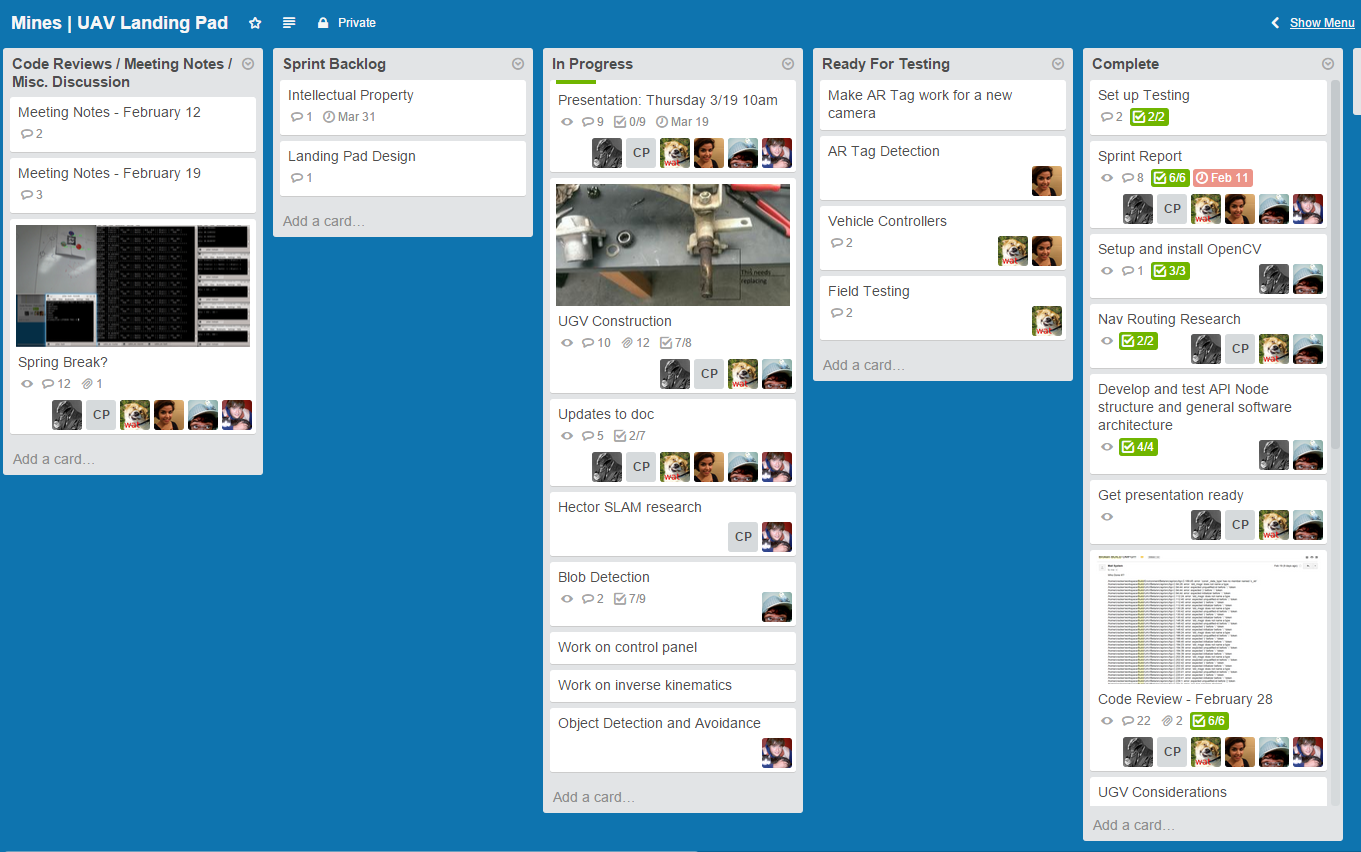
\includegraphics[width=1\textwidth]{resources/img/trello}
\end{center}
\caption{ UAV Landing Pad Team Trello Board. \label{apinode}}
\end{figure}


\subsubsection{Sprint Timeline}
Please refer to Table~\ref{sprinttimeline}, which details the entire sprint timeline for the UAV Landing Pad senior design project.

%I've separated everything out for your viewing pleasure ;)
\begin{table}[!bh]
\begin{tabular}{|| l || c | r || }
\hline
\textbf{Task}.............................................................................................. & \textbf{Start Date} & \textbf{End Date} \\
\hline
\hline
\textbf{Sprint 1} &  \textbf{09/15/14} & \textbf{10/03/14} \\
\hline
\hspace{15pt}Project Configuration & 09/15/14 & 09/20/14 \\
\hline
\hspace{15pt}Ubuntu 14.04 Installation & 09/15/14 & 09/16/14 \\
\hline
\hspace{15pt}ROS Installation, Configuration, \& Orientation & 09/16/14 & 10/03/14 \\
\hline
\hspace{15pt}Preliminary Technology Research & 09/15/14 & 10/08/14 \\
\hline
\hspace{30pt}\textit{S1 Summary} & 10/09/14   & 10/09/14 \\
\hline


\textbf{Sprint 2} & \textbf{10/13/14} & \textbf{10/31/14} \\
\hline
\hspace{15pt}OpenCV Installation \& Configuration & 10/21/14 & 10/22/14 \\
\hline
\hspace{15pt}Hardware stress test  &10/23/14  &10/29/14 \\
\hline
\hspace{15pt}LED Recognition/Detection &10/22/14  &10/24/14 \\
\hline
\hspace{15pt}SVO Decision & 10/27/14  &11/04/14 \\
\hline
\hspace{15pt}Repair Drone & 10/27/14  &11/04/14 \\
\hline
\hspace{30pt}\textit{Client Presentation} & 10/21/14 & 10/23/14 \\
\hline
\hspace{30pt}\textit{S2 Summary} & 11/06/14   & 11/06/14 \\
\hline


\textbf{Sprint 3}  &  \textbf{11/11/14} & \textbf{11/29/14} \\
\hline
\hspace{15pt}UGV Design Begins  &  11/13/14   & 12/05/14 \\
\hline
\hspace{15pt}GPS Research  &  11/11/14   & 11/11/14 \\
\hline
\hspace{15pt}Complete Architecture Design   & 11/11/14  &  11/12/14 \\
\hline
\hspace{15pt}Hector SLAM R\&D   & 11/14/14   & 12/01/14 \\
\hline
\hspace{30pt}\textit{Client Presentation}  &  12/02/14  &  12/02/14 \\
\hline
\hspace{30pt}\textit{S3 Summary}   & 12/05/14  &  12/05/14 \\
\hline


\textbf{Sprinter Break}  & \textbf{ 12/22/14 }  & \textbf{1/16/15} \\
\hline
\hspace{15pt}UGV Construction  &  12/22/14   & 12/29/14 \\
\hline
\hspace{15pt}OpenCV Homography  &  12/22/14   & 12/23/14 \\
\hline
\hspace{15pt}ROS Node Architecture Setup   & 12/29/14  &  01/2/15 \\
\hline
\hspace{15pt}Testing Environment Setup   & 12/29/14  &  01/16/15 \\
\hline


\textbf{Sprint 4}   & \textbf{01/19/15} & \textbf{02/06/15} \\
\hline
\hspace{15pt}Platform Design \& Development  &  01/30/15  &  02/11/15 \\
\hline
\hspace{15pt}UAV best case scenario landing  &  01/30/15  &  02/11/15 \\
\hline
\hspace{30pt}\textit{S4 Summary}  &  02/13/15   & 02/13/15 \\
\hline


\textbf{Sprint 5}   & \textbf{02/16/15} & \textbf{03/06/15} \\
\hline
\hspace{15pt}Finish UGV  &  02/13/15   & 03/16/15 \\
\hline
\hspace{15pt}Finish GPS \& NAV   & 02/13/15   & 03/09/15 \\
\hline
\hspace{15pt}Design Control Panel   & 02/13/15   & 03/16/15 \\
\hline
\hspace{15pt}Design UAV Flight Systems   & 03/02/15  &  03/16/15 \\
\hline
\hspace{15pt}Object Tracking ( OpenCV + AR )  &  02/13/15  &  3/13/15 \\
\hline
\hspace{30pt}\textit{Client Presentation}  &  03/19/15   & 03/19/15 \\
\hline
\hspace{30pt}\textit{S5 Summary}   & 03/20/15   & 03/20/15 \\
\hline


\textbf{Sprint 6}  &  \textbf{03/23/15} & \textbf{04/10/15} \\
\hline
\hspace{15pt}Component Integration   & 03/20/15  &  03/27/15 \\
\hline
\hspace{15pt}Integrate Control Panel  &  03/20/15 & 03/27/15 \\
\hline
\hspace{15pt}Handover Documents   & 03/23/15  &  05/07/15 \\
\hline
\hspace{15pt}Platform Implementation  &  03/30/15  &  04/10/15 \\
\hline
\hspace{15pt}Intensive Field Testings   & 03/30/15  &  04/29/15 \\
\hline
\hspace{30pt}\textit{S6 Summary}  &  04/10/15  &  04/10/15 \\
\hline
\hspace{30pt}\textit{Design Fair}  &  04/14/15   & 04/14/15 \\
\hline
\hspace{30pt}\textit{All Materials Due for Senior Design}  &  05/08/15  &  05/08/15 \\
\hline
\end{tabular}
\caption{ Sprint Timeline consisting of 6 Sprints and "Sprinter Break" \label{sprinttimeline}}
\end{table}




\subsubsection{Source Control}
The source code for our project is located on a private SVN repository provided by the Mathematics and Computer Science department at the South Dakota School of Mines and Technology. The repository is located at \url{http://dev.mcs.sdsmt.edu/repos/srdesign1415/robots/trunk/landingpad/}.


\section{User Stories}

The user stories section of this document describes the applications of this project in a real-life scenario point of view. This will allow stakeholders and anyone else interested or invested in this project to get a more explicit understanding of what we strive to accomplish with our fully autonomous system. Our user stores have been derived from design requirement meetings with our product owner, Dr. Jeff McGough. As such, all functional requirements of our system are described in the following sections.

\subsection{User Story \#1}
As a member of a search and rescue team, a volunteer will dedicate their time to saving lives, providing emergency assistance to those in need. Although members of search and rescue teams are certainly highly trained to operate in dangerous conditions, some scenarios, such as during massive forest fires in the Black Hills area, have an incredibly high risk of operational failure. Locations such as a large forest fire would be incredibly difficult for a human to navigate through; a lot of initial time would be wasted wandering through the forested area finding missing persons. Prolonged interactions within the forest fire will quickly put the members of the search and rescue team at risk.

\subsubsection{User Story \#1 Breakdown}
 A solution to the aforementioned user story would be to have a supplementary device capable of providing a bird's eye view of the dangerous location. This device would assist with finding missing person in areas of low radio communication and high human risk, therefore lowering the possibilities of casualties in the rescue mission, both missing persons and members of the rescue team.

Our project proposes to use a combination of a UAV and UGV to solve the problem stated in the user story. The UGV will autonomously drive to specified locations near the danger zone. The UAV will deploy from a landing pad situated on the UGV and collect sensor data of the danger zone from above in an attempt to determine if any missing persons are in the area. After the UAV has completed the flight, it will autonomously land back onto the UGV in order to recharge as the ground vehicle moves on to the next destination.

While this user story mainly focuses on the system handling a forest fire situation, our system could be applied to various other rescue missions in locations where human involvement from a rescue team should be kept at a minimum to avoid risking the lives of the team. Additional scenarios such as these include, but are not limited to:
\begin{itemize}
  \item Radioactive Locations
  \item Trench Rescues
  \item Mass Casualty Locations
  \item Water Rescue
  \item Other Natural Disaster Locations
\end{itemize}

\subsection{User Story \#2} 
User Story \#2 further elaborates on User Story \#1 but is done from the perspective of a member of the search and rescue team now using our UAV and UGV out on the field. As a search and rescue team member being assisted by our UAV and UGV, a minimal amount of user interaction must occur between the team member and UAV/UGV. The search and rescue team's first and foremost priority is to save lives, and any time spent fussing with hardware will be a severe detriment to their mission. Therefore, the UAV and UGV should be able to operate and navigate the area on their own accord.
 
\subsubsection{User Story \#2 Breakdown}
This user story describes the necessity of an autonomous system. The ground vehicle will handle path planning through GPS and point cloud data. GPS will determine the various waypoints for the UGV's route. Point cloud data will be utilized to determine how close any large objects are to the ground vehicle. This will allow the UGV to have an understanding of the environment without having a human controlling the vehicle's steering. Event-handling routines will allow the ground vehicle to modify its navigation path to accommodate any unexpected obstacles in its original path. 

The user story also provides the specification that the UAV and UGV must be able to communicate with one another. This requirement is accomplished with the ROS environment, which is build with a very extensive yet simple message passing communication system. This publish/subscribe mechanism works well not only for intercommunication between various components on board each vehicle, but also allows synchronization between the UAV and UGV. Because of the asynchronous behavior of the publisher/subscriber system, the UGV can send commands to the UAV to initiate flight once the ground vehicle has reached a destination waypoint.


%\subsection{User Story \#3} 
%\subsubsection{User Story \#3 Breakdown}
%User story \#3  .... 


\section{Research or Proof of Concept Results}
Sprints 1, 2, and 3 involved an extensive amount of research into what different components we would explore in order to accomplish autonomy of a hardware system. For the UGV, obstacle avoidance would be our greatest challenge in our navigation algorithms. For the UAV, autonomously landing the UAV onto the small landing pad situated on the back of our ground vehicle would prove to be a challenge.

\subsection{UGV - Point Cloud Research}
Point clouds are a set of data points in a given (x,y,z) coordinate system, often created by a 3D scanning system. The team's initial research into point cloud data was in order to establish a mapping system by registering a dense point cloud map of the environment and planning navigation and object avoidance based off of the mapped data. 

\begin{figure}[!h]
\begin{center}
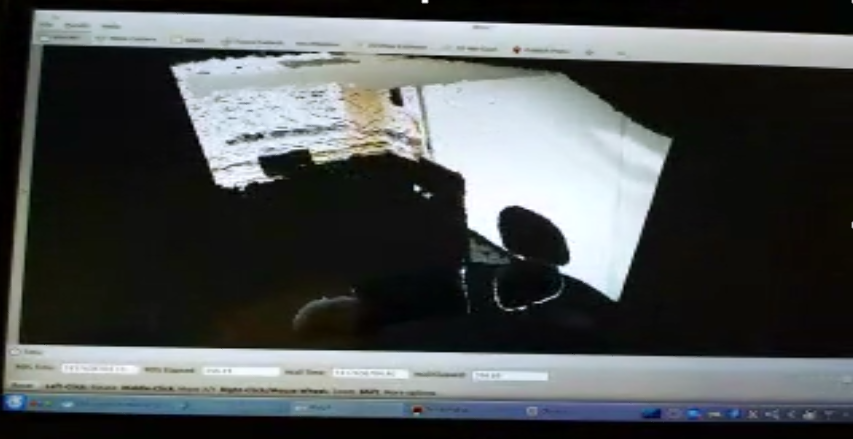
\includegraphics[width=0.5\textwidth]{resources/img/point_cloud}
\end{center}
\caption{Point cloud data of \ McLaury Room 108.\label{pointcloud108}}
\end{figure}

Using an Asus Xtion Live Pro, which communicates to ROS through openni2, point cloud data can be read in and stored as a 2D vector. This vector can be searched to find if any objects were detected within a certain distance in front of the vehicle, approximately 4 meters or however far the ground vehicle's object avoidance methods need to be calibrated. Each frame of the point cloud data is analyzed to determine any obstacles coming towards the ground vehicle.




\subsection{UAV - OpenCV Research}
One of the main challenges in designing the autonomous UAV was determining how the aircraft would handle landing onto the ground vehicle after completing a flight. The solution to this challenge was to use OpenCV, an open-source computer vision library. OpenCV would allow us to use object recognition routines to recognize the landing pad, allowing the autonomous UAV to verify the landing pad is within the aircraft's "vision".

\begin{figure}[!h]
\begin{center}
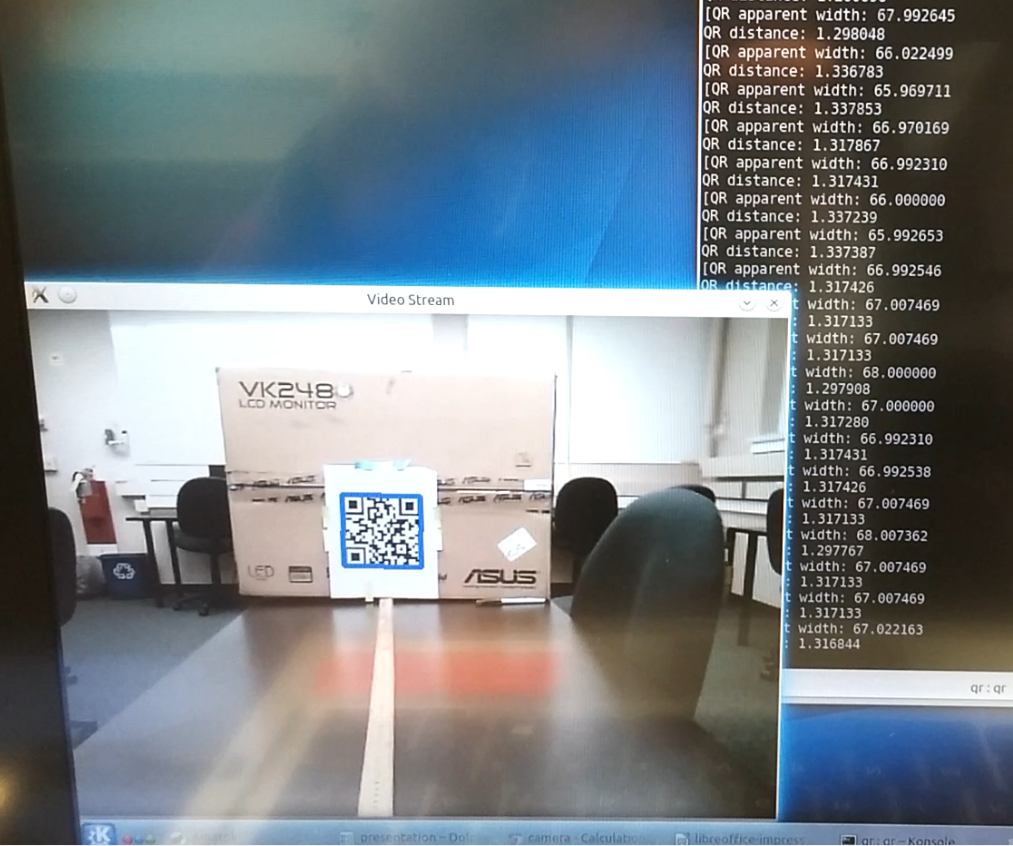
\includegraphics[width=.8\textwidth]{resources/img/qr}
\end{center}
\caption{QR Code tracking in openCV.\label{qr}}
\end{figure}

The initial proof of concept test for recognition was to use the Zbar open source barcode library to see if the team could track a qr code with a camera and determine the code's distance from the camera. The qr code was printed and mounted approximately 1.3 meters from the camera, which successfully tracked the code and output the calculated distance based on the camera's focal length and the known size of the printed qr code. The formulas utilized to determine object distance based on camera focal length and the observed size of a known object are detailed in Subsection~\ref{cvtracker}.

The results of this initial research were that the team could certainly utilize openCV as a tracking routine that also returned distance from the tracked object. However, landing the aircraft is still an incredibly complicated and important component of this system, so a redundant system would be desired for returning the aircraft's distance from the landing pad. Therefore, the openCV tracking was shifted away from tracking qr codes and refocused on tracking multiple colored objects in a specified triangular pattern on the landing pad. 


\begin{figure}[!h]
\begin{center}
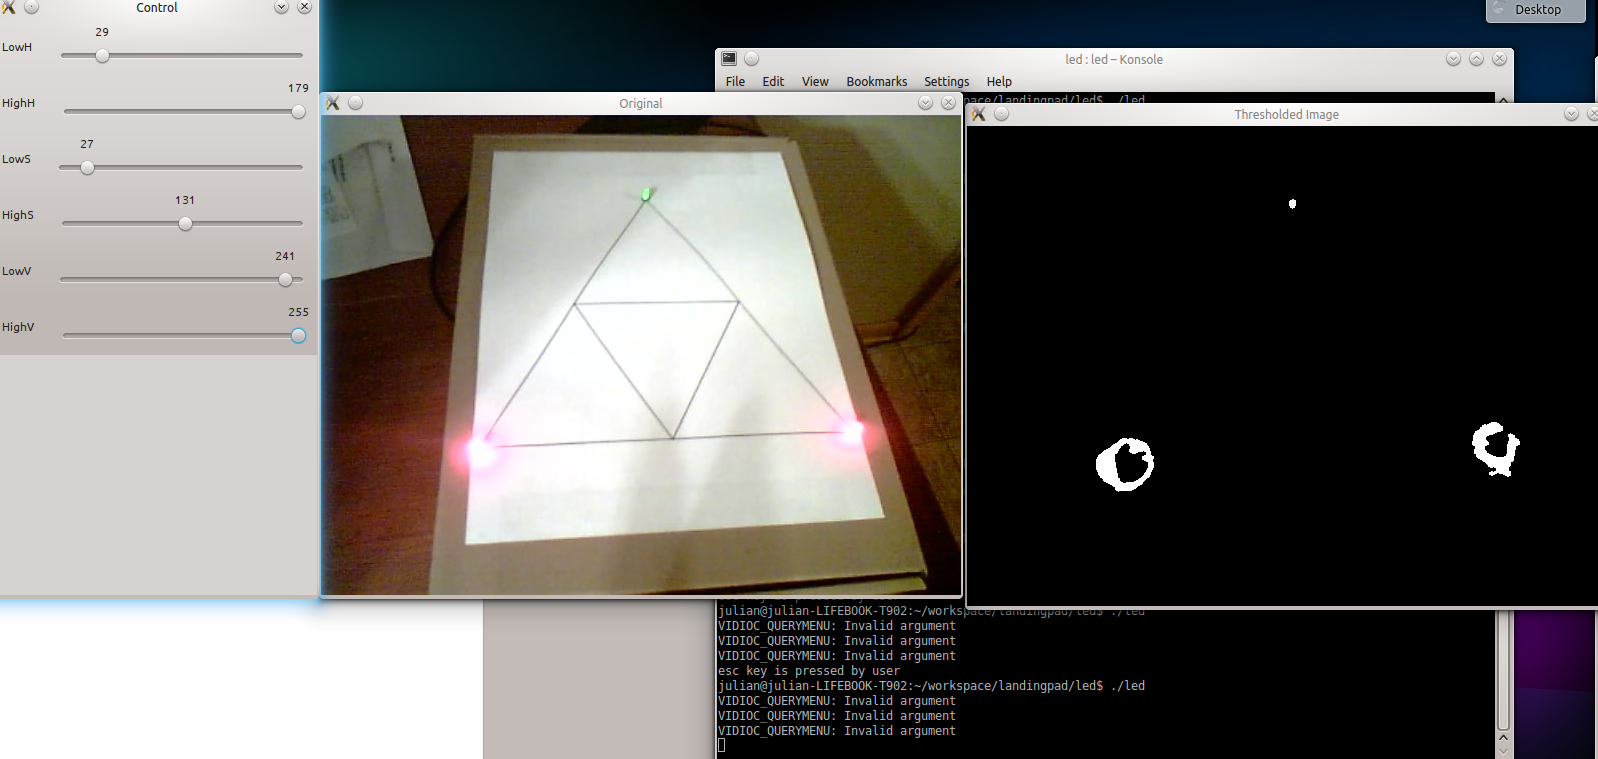
\includegraphics[width=0.5\textwidth]{resources/img/ledtracking01}
\end{center}
\caption{LED tracking in openCV.\label{ledtracking}}
\end{figure}

At one point during Sprint \#2, a tracking system using three colored LEDs was investigated. However, complications arose due to the fact that the emissive quality of the LEDs caused the lights to produce a non-uniform color. An artifact of this time of development is evident in the naming conventions of some of the classes in the cv\_tracker ROS package. The final design of the landing pad is three colored circles printed onto the landing pad design. Tracking multiple objects introduced multiple distance readings, rather than relying on one potentially unstable distance reading. ROS's AR tag tracking capabilities were also incorporated in conjunction with the openCV tracking system to create a sophisticated and thorough craft orientation and landing routine. Further actualization of this initial research can be detailed in Section~\ref{softwarecraftorientation}.






%\section{Supporting Material}


%This document might contain references or supporting material which should be documented 
%and discussed  either here if appropriate or more often in the appendices at the end.  This material may have been provided by the stakeholders  
%or it may be material garnered from research tasks.

